% =============================================================================
%  T5 / P1 - Simulador de Espelho Corporal (Tema 6)
%  Processamento de Imagens - UFMA
%
%  9 slides, curtos. Figuras geradas por:  python apresentacao/gerar_figuras.py
%  Compilar com XeLaTeX:  latexmk -xelatex apresentacao.tex
% =============================================================================

\documentclass[aspectratio=169,12pt]{beamer}

% -----------------------------------------------------------------------------
%  >>> PREENCHA AQUI <<<
% -----------------------------------------------------------------------------
\newcommand{\alunos}{ANDRE LUIS AGUIAR DO NASCIMENTO \\
JOAO GUILHERME MIRANDA LAGO \\
WESLEY DOS SANTOS GATINHO}
\newcommand{\professor}{Prof. HAROLDO GOMES BARROSO FILHO}
% -----------------------------------------------------------------------------

\usetheme[progressbar=none, numbering=fraction, block=fill]{metropolis}

\usepackage{fontspec}
\setsansfont{Fira Sans}[Numbers=Lining]
\setmonofont{Fira Mono}[Scale=0.82]
\usepackage[brazil]{babel}
\usepackage{amsmath}
\usepackage{booktabs}
\usepackage{graphicx}
\usepackage{tikz}
\usetikzlibrary{arrows.meta, positioning}

\graphicspath{{figuras/}}

\definecolor{ink}{HTML}{16262E}
\definecolor{cinza}{HTML}{5A6B73}
\definecolor{papel}{HTML}{FAFAF8}
\definecolor{marca}{HTML}{9A3B26}
\definecolor{lite}{HTML}{2A78D6}
\definecolor{full}{HTML}{EB6834}

\setbeamercolor{normal text}{fg=ink, bg=papel}
\setbeamercolor{alerted text}{fg=marca}
\setbeamercolor{frametitle}{bg=ink, fg=papel}
\setbeamercolor{title separator}{fg=marca}
\setbeamerfont{frametitle}{size=\large}
\setbeamertemplate{itemize items}[circle]
\setlength{\parskip}{.35em}

\newcommand{\leg}[1]{{\small\textcolor{cinza}{#1}}}

% Figura feita a partir do video gravado. Se ainda nao existir, mostra um
% espaco reservado com a instrucao para gera-la.
%   uso: \figuravideo{largura}{altura do espaco}{arquivo}
\newcommand{\figuravideo}[3]{%
  \IfFileExists{figuras/#3.png}{\includegraphics[width=#1]{#3}}{%
    \fcolorbox{cinza}{white}{\parbox[c][#2][c]{\dimexpr#1-2\fboxsep-2\fboxrule\relax}{\centering
      \textcolor{cinza}{\small Figura \texttt{\detokenize{#3}.png}: grave um vídeo e rode\\
      \texttt{python apresentacao/gerar\_figuras.py}}}}}}

\title{Simulador de Espelho Corporal}
\subtitle{Estimativa de pose em tempo real com MediaPipe e OpenCV}
\author{\alunos}
\institute{Processamento de Imagens \\ Universidade Federal do Maranhão \\ \professor}
\date{Trabalho T5 · Tema 6}

\begin{document}

\maketitle

% =============================================================================
\begin{frame}{Objetivo e arquitetura}

  Reproduzir os movimentos da pessoa, com o esqueleto desenhado em tempo real.

  \vspace{.5em}
  \begin{center}
  \begin{tikzpicture}[
      caixa/.style={draw=ink, rounded corners=3pt, line width=.7pt, align=center,
                    minimum height=1.3cm, text width=1.62cm, font=\footnotesize, fill=white},
      sub/.style={font=\scriptsize, text=cinza},
      seta/.style={-{Stealth[length=2mm]}, line width=.8pt, draw=marca},
      node distance=.32cm]
    \node[caixa] (cam) {Webcam\\{\scriptsize\color{cinza}30 FPS}};
    \node[caixa, right=of cam] (cv) {OpenCV\\{\scriptsize\color{cinza}captura}};
    \node[caixa, right=of cv] (mp) {MediaPipe\\Pose\\{\scriptsize\color{cinza}Lite · Full · Heavy}};
    \node[caixa, right=of mp] (lm) {33\\landmarks\\{\scriptsize\color{cinza}x, y, z, visib.}};
    \node[caixa, right=of lm] (fx) {Espelho\\+ filtro\\{\scriptsize\color{cinza}One Euro}};
    \node[caixa, right=of fx] (tela) {Esqueleto\\na tela};
    \foreach \a/\b in {cam/cv, cv/mp, mp/lm, lm/fx, fx/tela} \draw[seta] (\a) -- (\b);
  \end{tikzpicture}
  \end{center}

  \vspace{.3em}
  \begin{itemize}
    \item Três modelos pré-treinados, trocáveis com o programa aberto.
    \item O próprio programa mede FPS, latência, acerto e estabilidade.
  \end{itemize}

\end{frame}

% =============================================================================
\begin{frame}{O espelho}

  \begin{center}
    \figuravideo{.9\textwidth}{4.2cm}{modos}
  \end{center}

  \vspace{-.7em}
  \begin{itemize}\small
    \item Detecta no quadro original e só depois espelha a imagem e faz $x \to 1-x$:
      assim esquerda e direita continuam corretas.
    \item Pontos com visibilidade $< 0{,}5$ (fora do quadro ou encobertos) não são desenhados.
  \end{itemize}

\end{frame}

% =============================================================================
\begin{frame}{Desempenho: FPS e latência}

  \begin{center}
    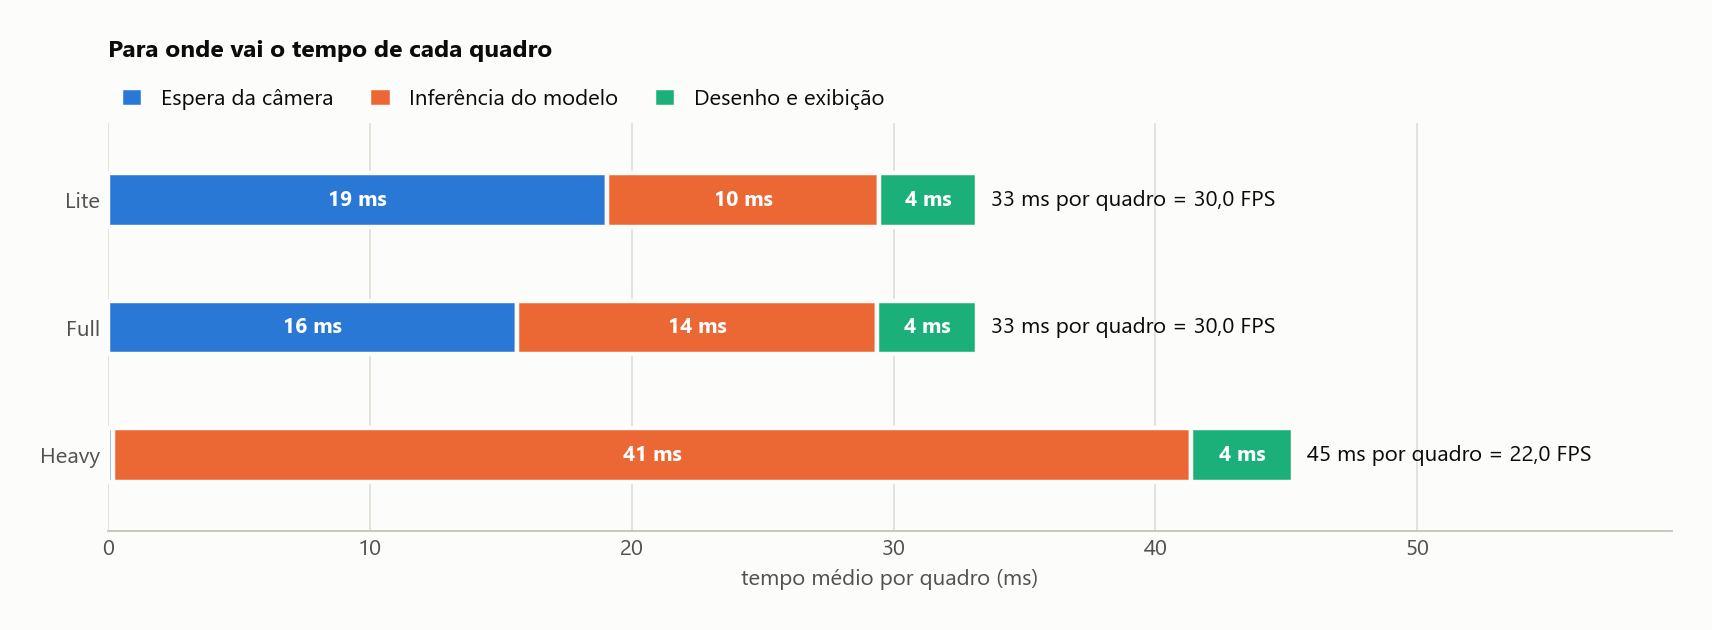
\includegraphics[width=.95\textwidth]{tempo_por_quadro}
  \end{center}

  \vspace{-.9em}
  {\small \textbf{Lite e Full}: o limite é a câmera, 30~FPS. \textbf{Heavy}: 41~ms de inferência
  não cabem nos 33~ms entre dois quadros.}

  \vspace{-.3em}
  \leg{Latência, do quadro chegar até aparecer na tela: 14, 18 e 45~ms.}

\end{frame}

% =============================================================================
\begin{frame}{Estabilidade}

  \begin{center}
    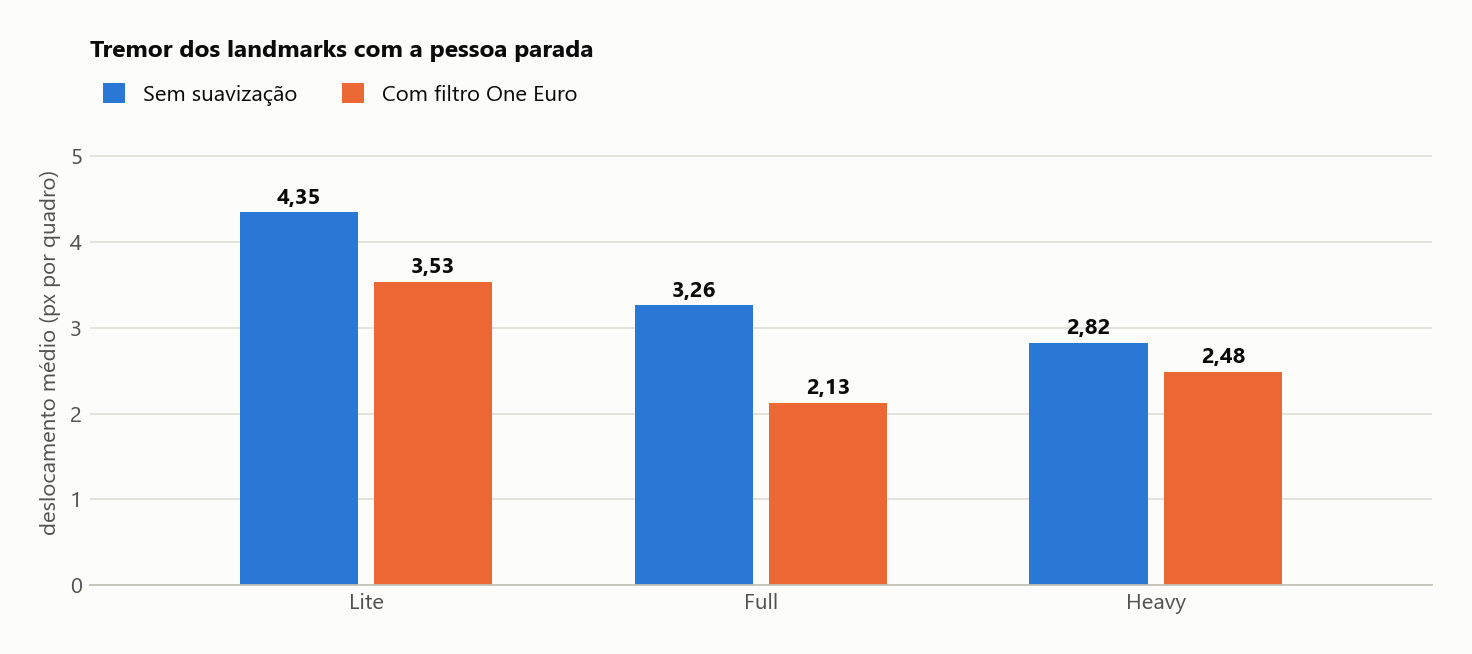
\includegraphics[width=.74\textwidth]{estabilidade}
  \end{center}

  \vspace{-.9em}
  {\small O filtro One Euro reduz o tremor em \textbf{19\,\%}, \textbf{35\,\%} e
  \textbf{12\,\%}, quase sem atrasar movimentos rápidos. Pose detectada em \textbf{100\,\%} dos quadros.}

  \vspace{-.3em}
  \leg{Tremor: quanto os pontos se mexem de um quadro para outro com a pessoa parada.}

\end{frame}

% =============================================================================
\begin{frame}{Taxa de acerto}

  Sem gabarito anotado à mão, o \textbf{Heavy} é a referência. Um ponto está correto se
  \[
    \lVert p - p_{\text{Heavy}} \rVert \;\le\; 0{,}2 \times \text{comprimento do tronco}
    \qquad \text{(PCK@0,2)}
  \]

  \vspace{-.3em}
  \begin{center}
  \begin{tabular}{lrr}
    \toprule
    Vídeo gravado (40~s, 8 poses) & \textcolor{lite}{\textbf{Lite}} & \textcolor{full}{\textbf{Full}} \\
    \midrule
    Perto, só a parte de cima do corpo & 99,8\,\% & 99,9\,\% \\
    Corpo inteiro, todas as poses      & 84,3\,\% & 92,2\,\% \\
    \quad de perfil                    & 56,2\,\% & 96,8\,\% \\
    \quad em uma perna                 & 35,2\,\% & 100,0\,\% \\
    \bottomrule
  \end{tabular}
  \end{center}

  \leg{Mede concordância com o modelo mais preciso, não acerto absoluto: um erro
  que os três modelos cometem juntos não aparece.}

\end{frame}

% =============================================================================
\begin{frame}{Onde o Lite falha}

  \begin{center}
    \figuravideo{.8\textwidth}{5.2cm}{lite_vs_full}
  \end{center}

  \vspace{-.6em}
  \leg{Em branco, o Heavy. De lado e em uma perna, o Lite junta a perna levantada com a de apoio; o Full acompanha.}

\end{frame}

% =============================================================================
\begin{frame}{Conclusões}

  \begin{itemize}
    \item \textbf{Full} é o melhor equilíbrio para o espelho: 30~FPS, 18~ms de latência,
      o menor tremor com filtro e 92\,\% de acerto de corpo inteiro.
    \item \textbf{Heavy} é o mais preciso, mas cai para 22~FPS.
    \item \textbf{Lite} é o mais rápido, mas erra em poses de lado e em uma perna.
    \item \textbf{Enquadramento} pesa tanto quanto o modelo: com o corpo cortado,
      até o Heavy erra.
  \end{itemize}

  \vspace{.3em}
  \leg{Limitações: uma gravação por cenário; a referência é o Heavy, não um gabarito;
  na pose ``braços para cima'' a cabeça saiu do quadro e a referência falhou.}

\end{frame}

% =============================================================================
\begin{frame}[standout]

  Demonstração

  \vspace{.8em}
  {\normalsize\mdseries
  \textbf{1}–\textbf{4} modos \qquad
  \textbf{L F H} modelo \qquad
  \textbf{S} suavização \qquad
  \textbf{Q} sair}

\end{frame}

\end{document}
